\chapter{RabbitMQ Server 启动机制}

\section{源码目录结构} 
 
RabbitMQ Server本质上是一个OTP Application,他有着典型的OTP app目录结构, 如图\ref{Fig:ch1/directory}:
\begin{figure}[h]
	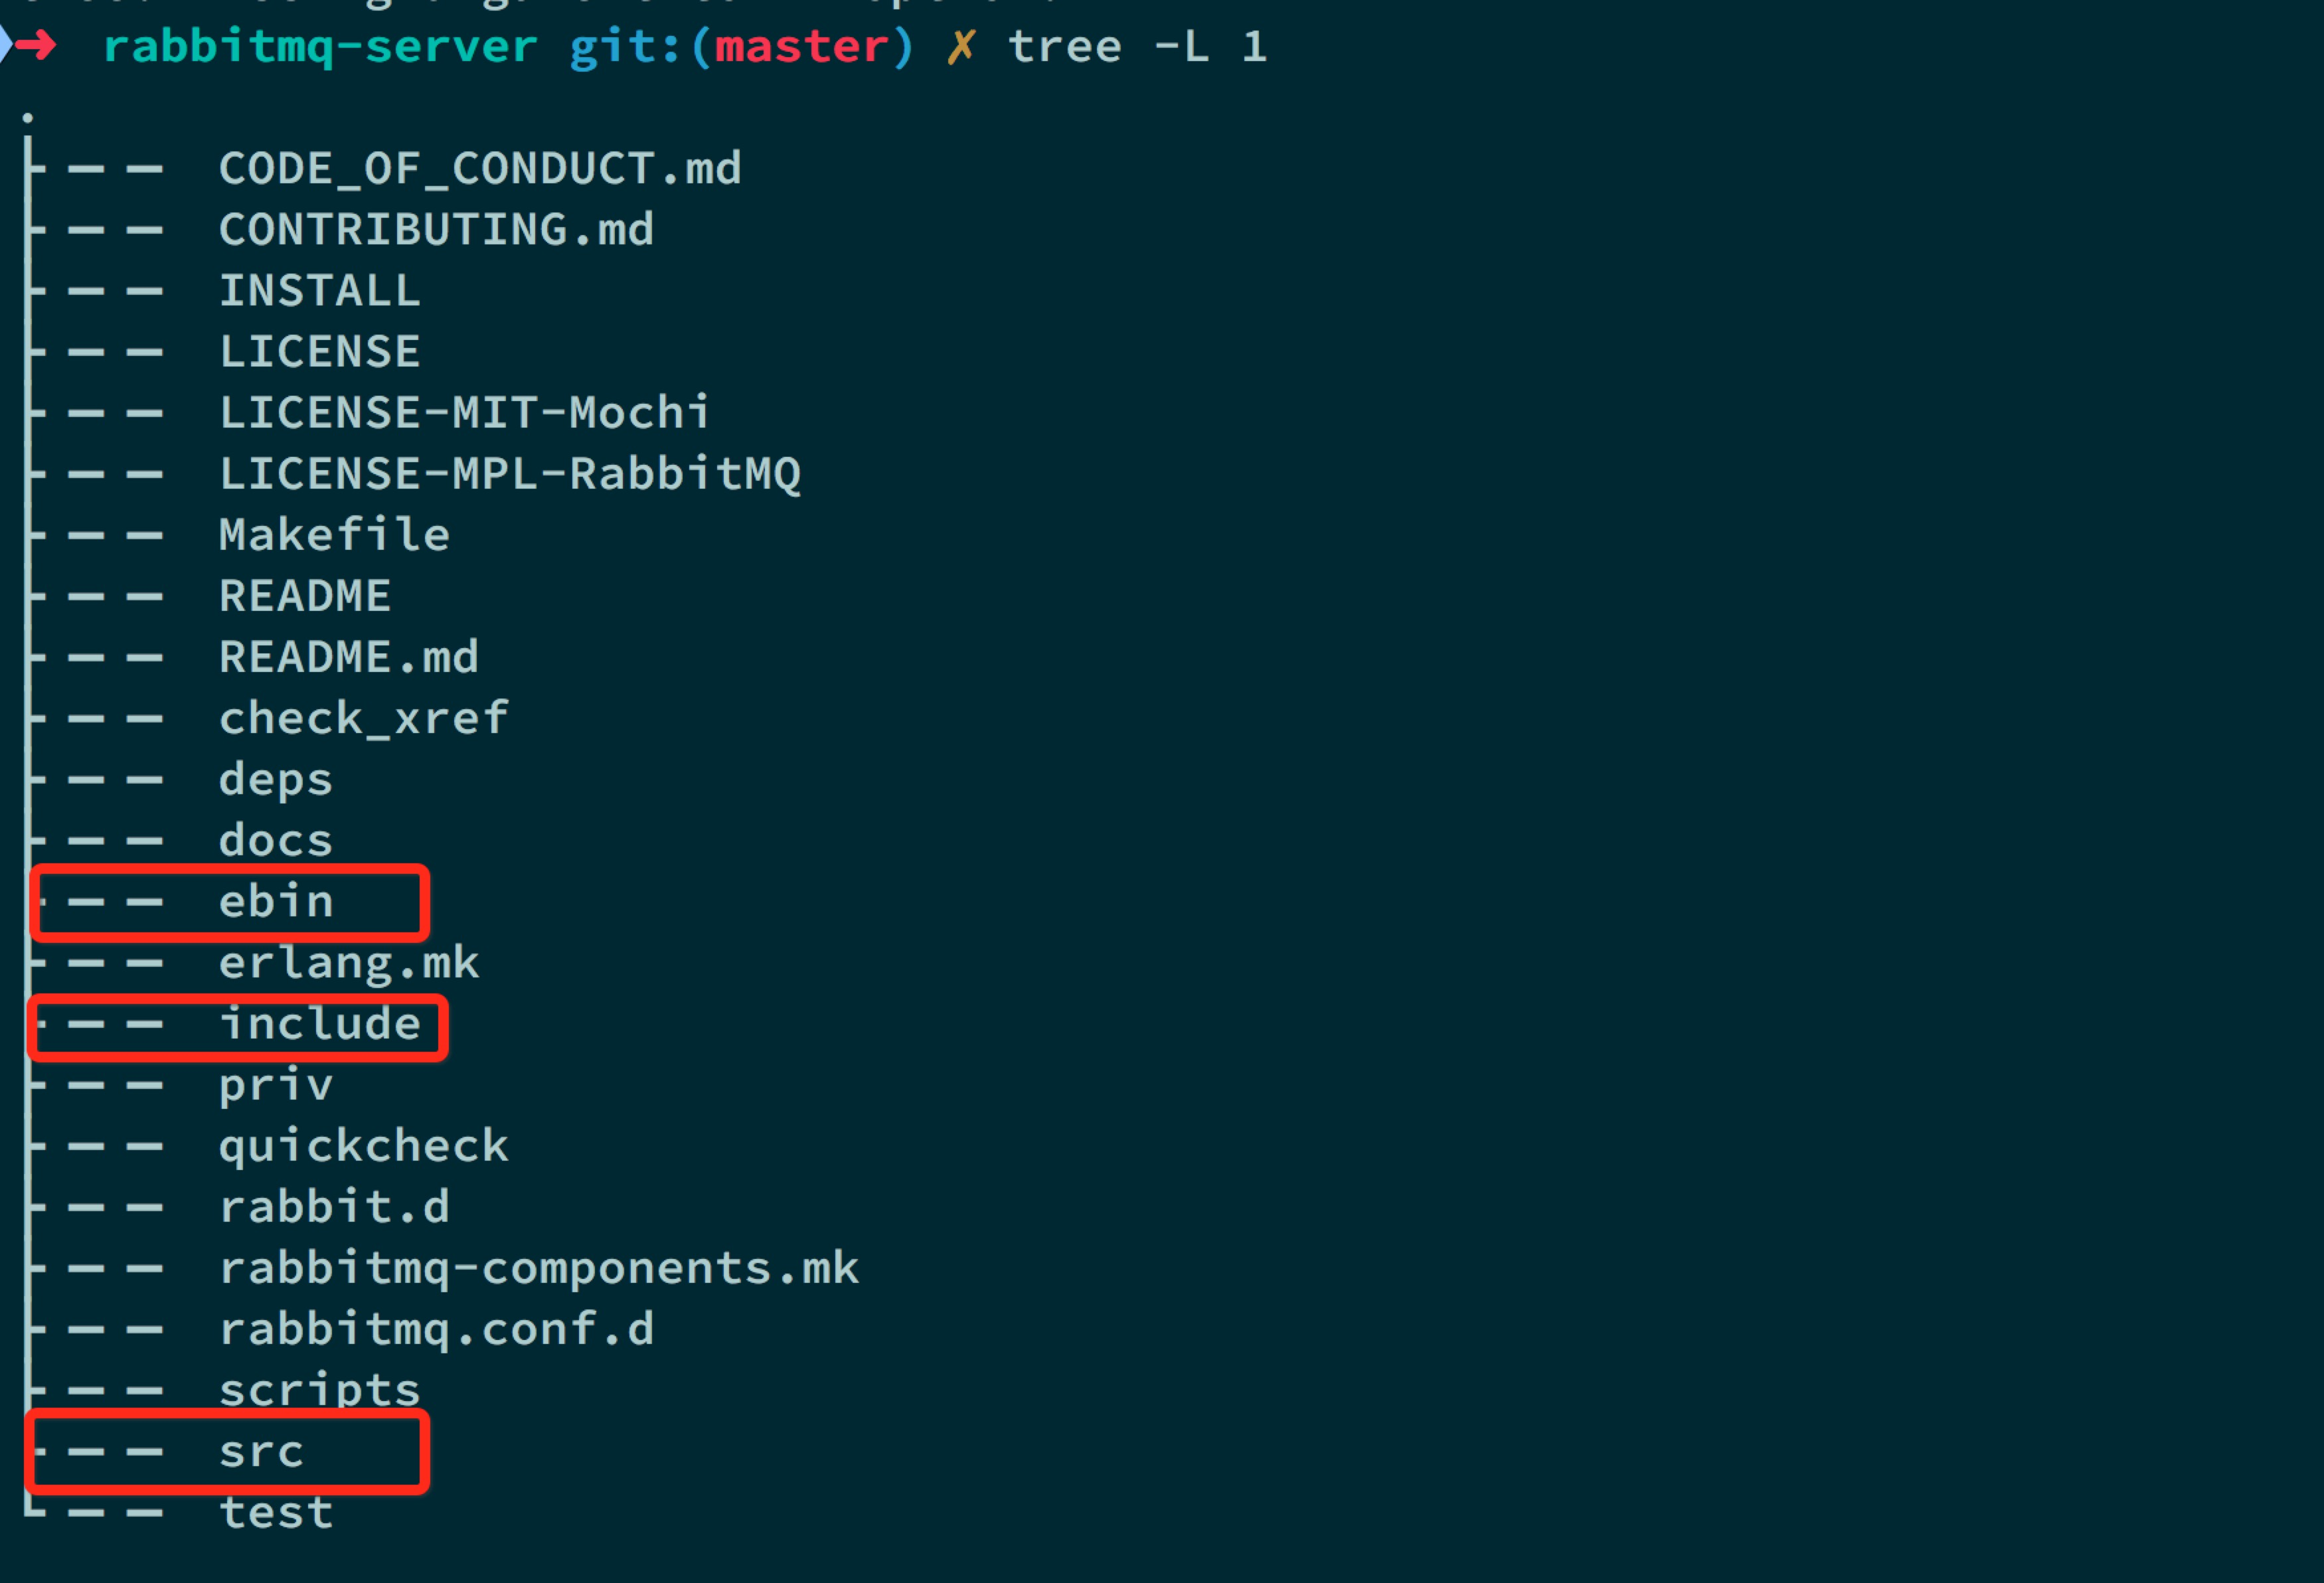
\includegraphics[height=8cm]{img/ch1/directory.jpeg}
	\caption{\label{Fig:ch1/directory}目录结构}
\end{figure}

在这个一级目录中红色方框中的目录是一个典型的OPT app目录。src主要是源码目录;ebin主要是erlang编译出的字节码文件,该目录还存放有一个重要的应用资源文件(AppName.app);include存放一些头文件,主要是一些record和宏定义。

\section{资源文件} 
因为资源文件ebin/rabbit.app定义了一个应用的基本资源信息, 所以我们首先来看下这个文件的内容, 如图\ref{Fig:ch1/rabbit_app}:
\begin{figure}[h]
	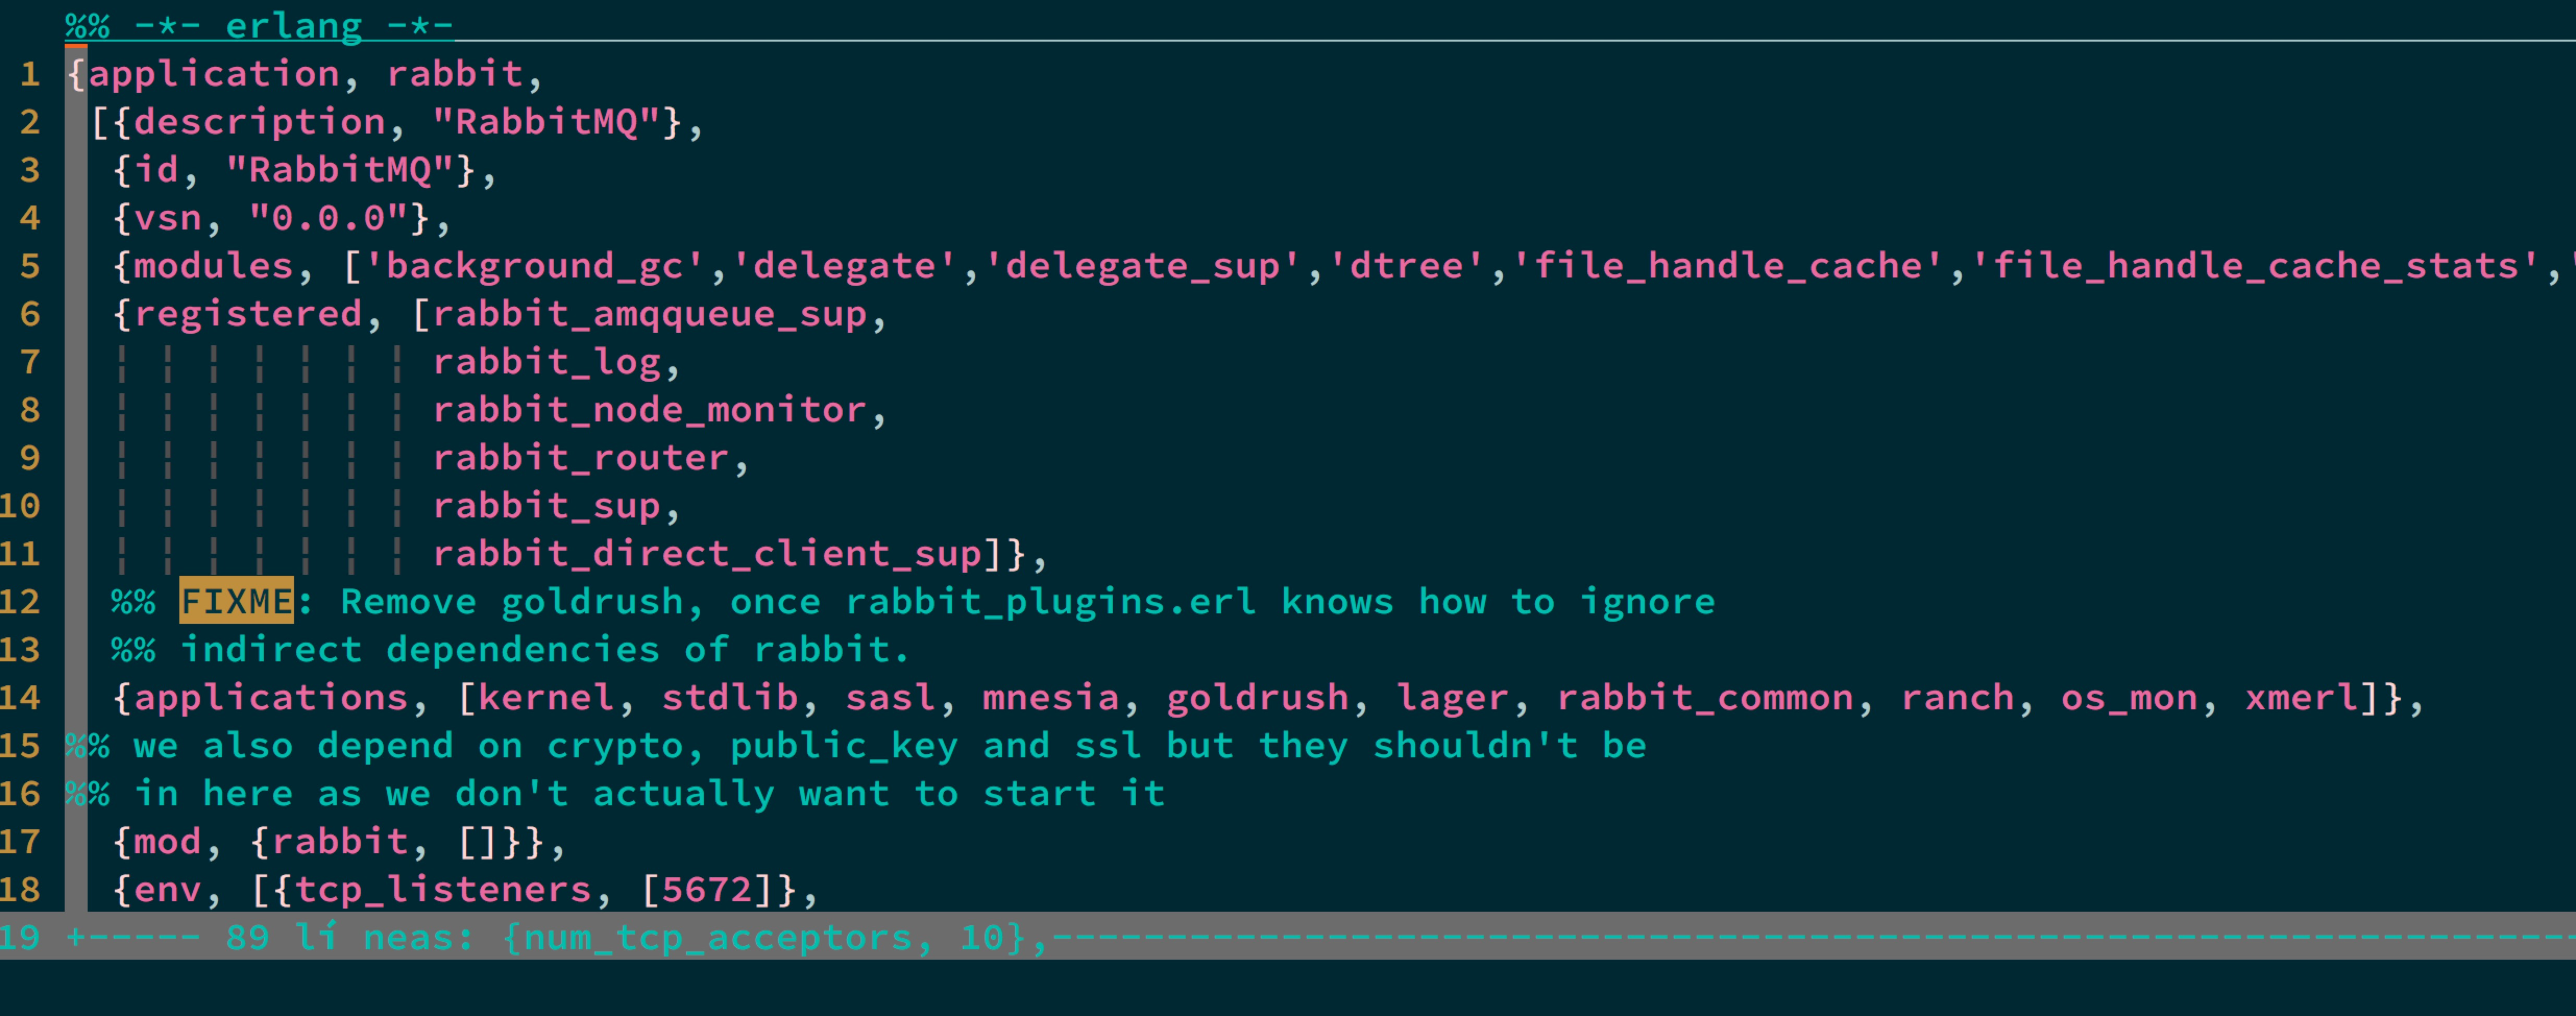
\includegraphics[height=10cm]{img/ch1/rabbit_app.jpeg}
	\caption{\label{Fig:ch1/rabbit_app}rabbit.app}
\end{figure}

资源文件其实就是erlang中的一个tuple数据类型; 出了1-5行主要定义了应用的名字、版本、描述等基本信息外;值得说明是的第五行{modules, ...}罗列了rabbitmq中的所有module模块。 第6️行{registered, ...}罗列了rabbit这个应用所启动的所有进程,这里有一个Erlang/TOTP很重要的设计模式Supervision Principles,基于该特性使得erlang可以很轻易的监测到进程的crash,并很轻易的重新启动新进程,从而丢弃了大多数语言的防御式编程模式,提出了”就让它崩溃吧“(let it crash),Orz...。 第10行的rabbit\_sup就是整个rabbit supervision tree的根;第11行定义了rabbit应用所依赖的其他应用。\textbf{第12行定义了application behavior的回调模块,这个模块的start(Type, StartArgs)就是整个应用程序的入口, 相当于main}。第18行{env,...}定义和应用的环境变量,rabbit的各个配置都可以在这里设置,鉴于篇幅问题没有展开剩下的环境变量;当然这些变量也可以通过命令行或者配置文件rabbitmq.config进行修改。


\section{启动流程}
根据前面的分析, 我们知道application behavior的程序入口是./src/rabbit.erl中start/2函数,如图\ref{Fig:ch1/start}
\begin{figure}[h]
	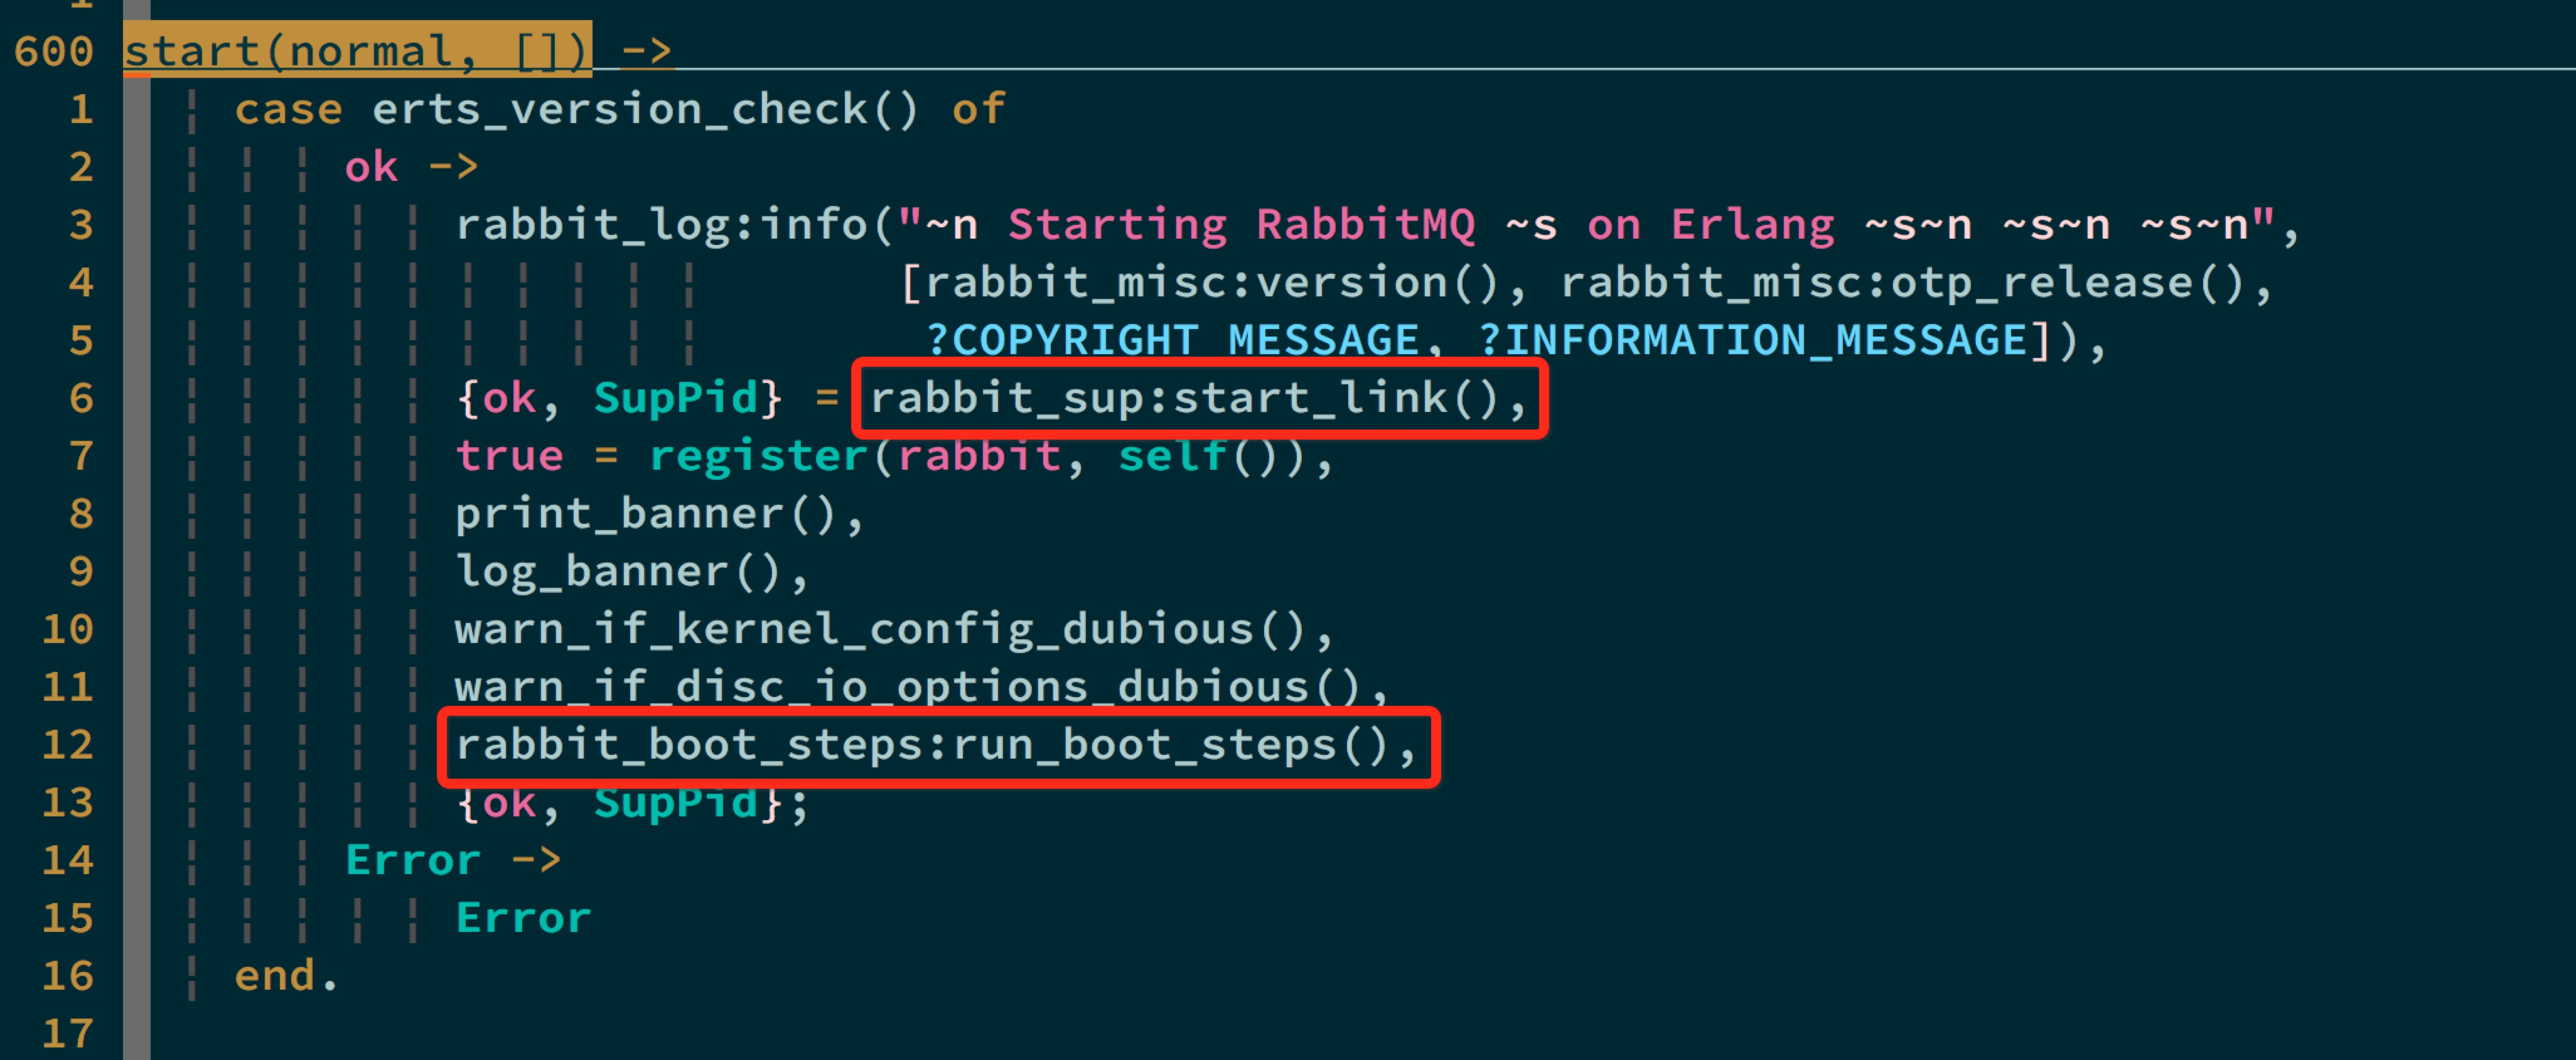
\includegraphics[height=10cm]{img/ch1/start.jpeg}
	\caption{\label{Fig:ch1/start}启动程序入口}
\end{figure}

该函数其实做了主要住了两件事:第一是创建一个supervision tree,这里的rabbit\_sup实现了supervisor behavior。 第二个是是重中之重,rabbitmq启动方式是通过boot\_step的方式启动, 在每个app中都定义了自己的boot\_step; 这个的boot\_step定义个待启动模块的方式,前驱依赖和后继依赖,理解为一个DAG图的一条边就好了,下面是一个列子:\ref{Fig:ch1/boot_step}
\begin{figure}[h]
	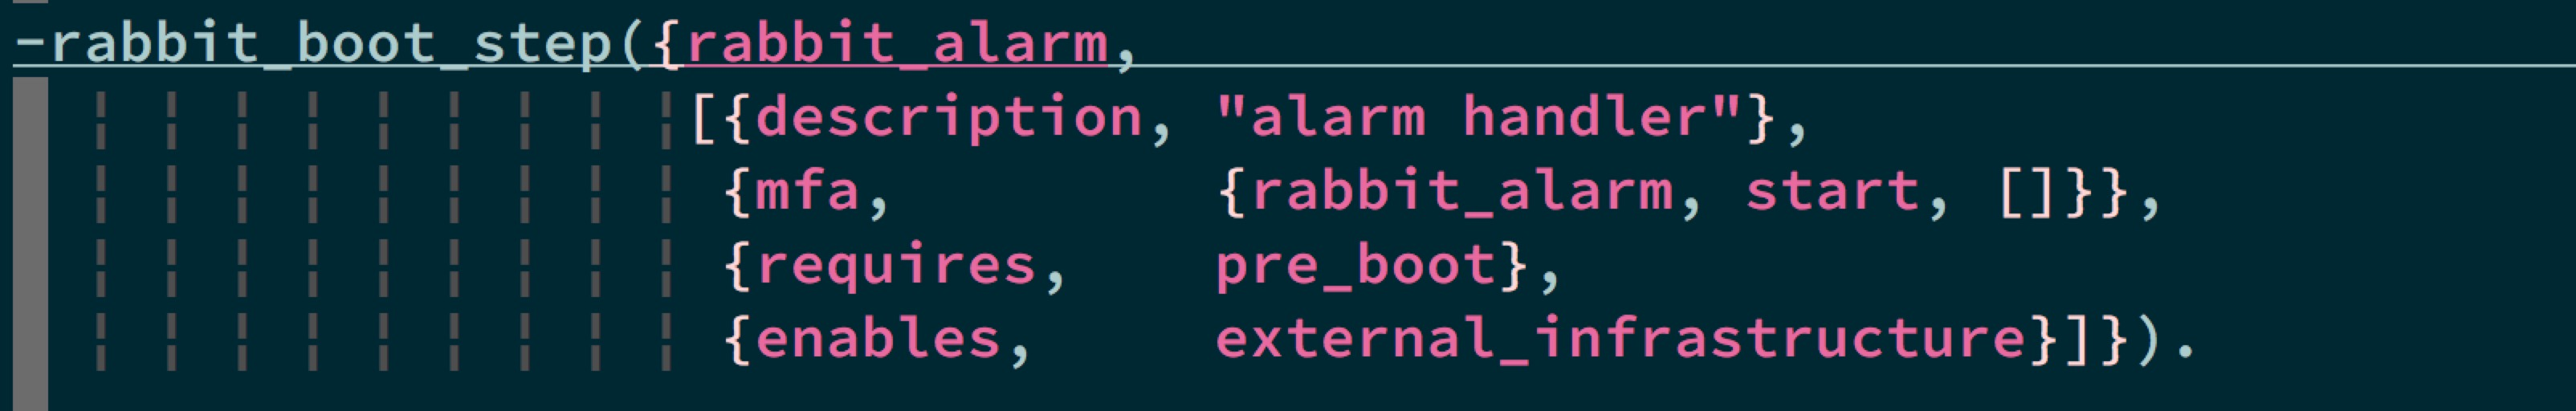
\includegraphics[width=\textwidth]{img/ch1/boot_step.jpeg}
	\caption{\label{Fig:ch1/boot_step}boot\_step例子}
\end{figure}

前两行定义了这个step的名字和描述,mfa是(module, function, arguments)的缩写,定义了如何启动这个step; requires指定了启动这个step所以依赖的前置条件, 也就是必须等requires中的module都启动完毕才能启动这个step;enables指定了启动这个step之后就可以解锁的module;

在图\ref{Fig:ch1/start}的第12行中,通过rabbit\_boot\_steps模块来启动所有的steps;从资源文件中我们知道rabbitmq有多个application,而每个application都有自己的boot\_step, 所以必须有一个单独的tool能够把这些组织在一起, 就是rabbit\_boot\_steps啦, 如图\ref{Fig:ch1/run_step} :
\begin{figure}[h]
	\vspace{0mm}
	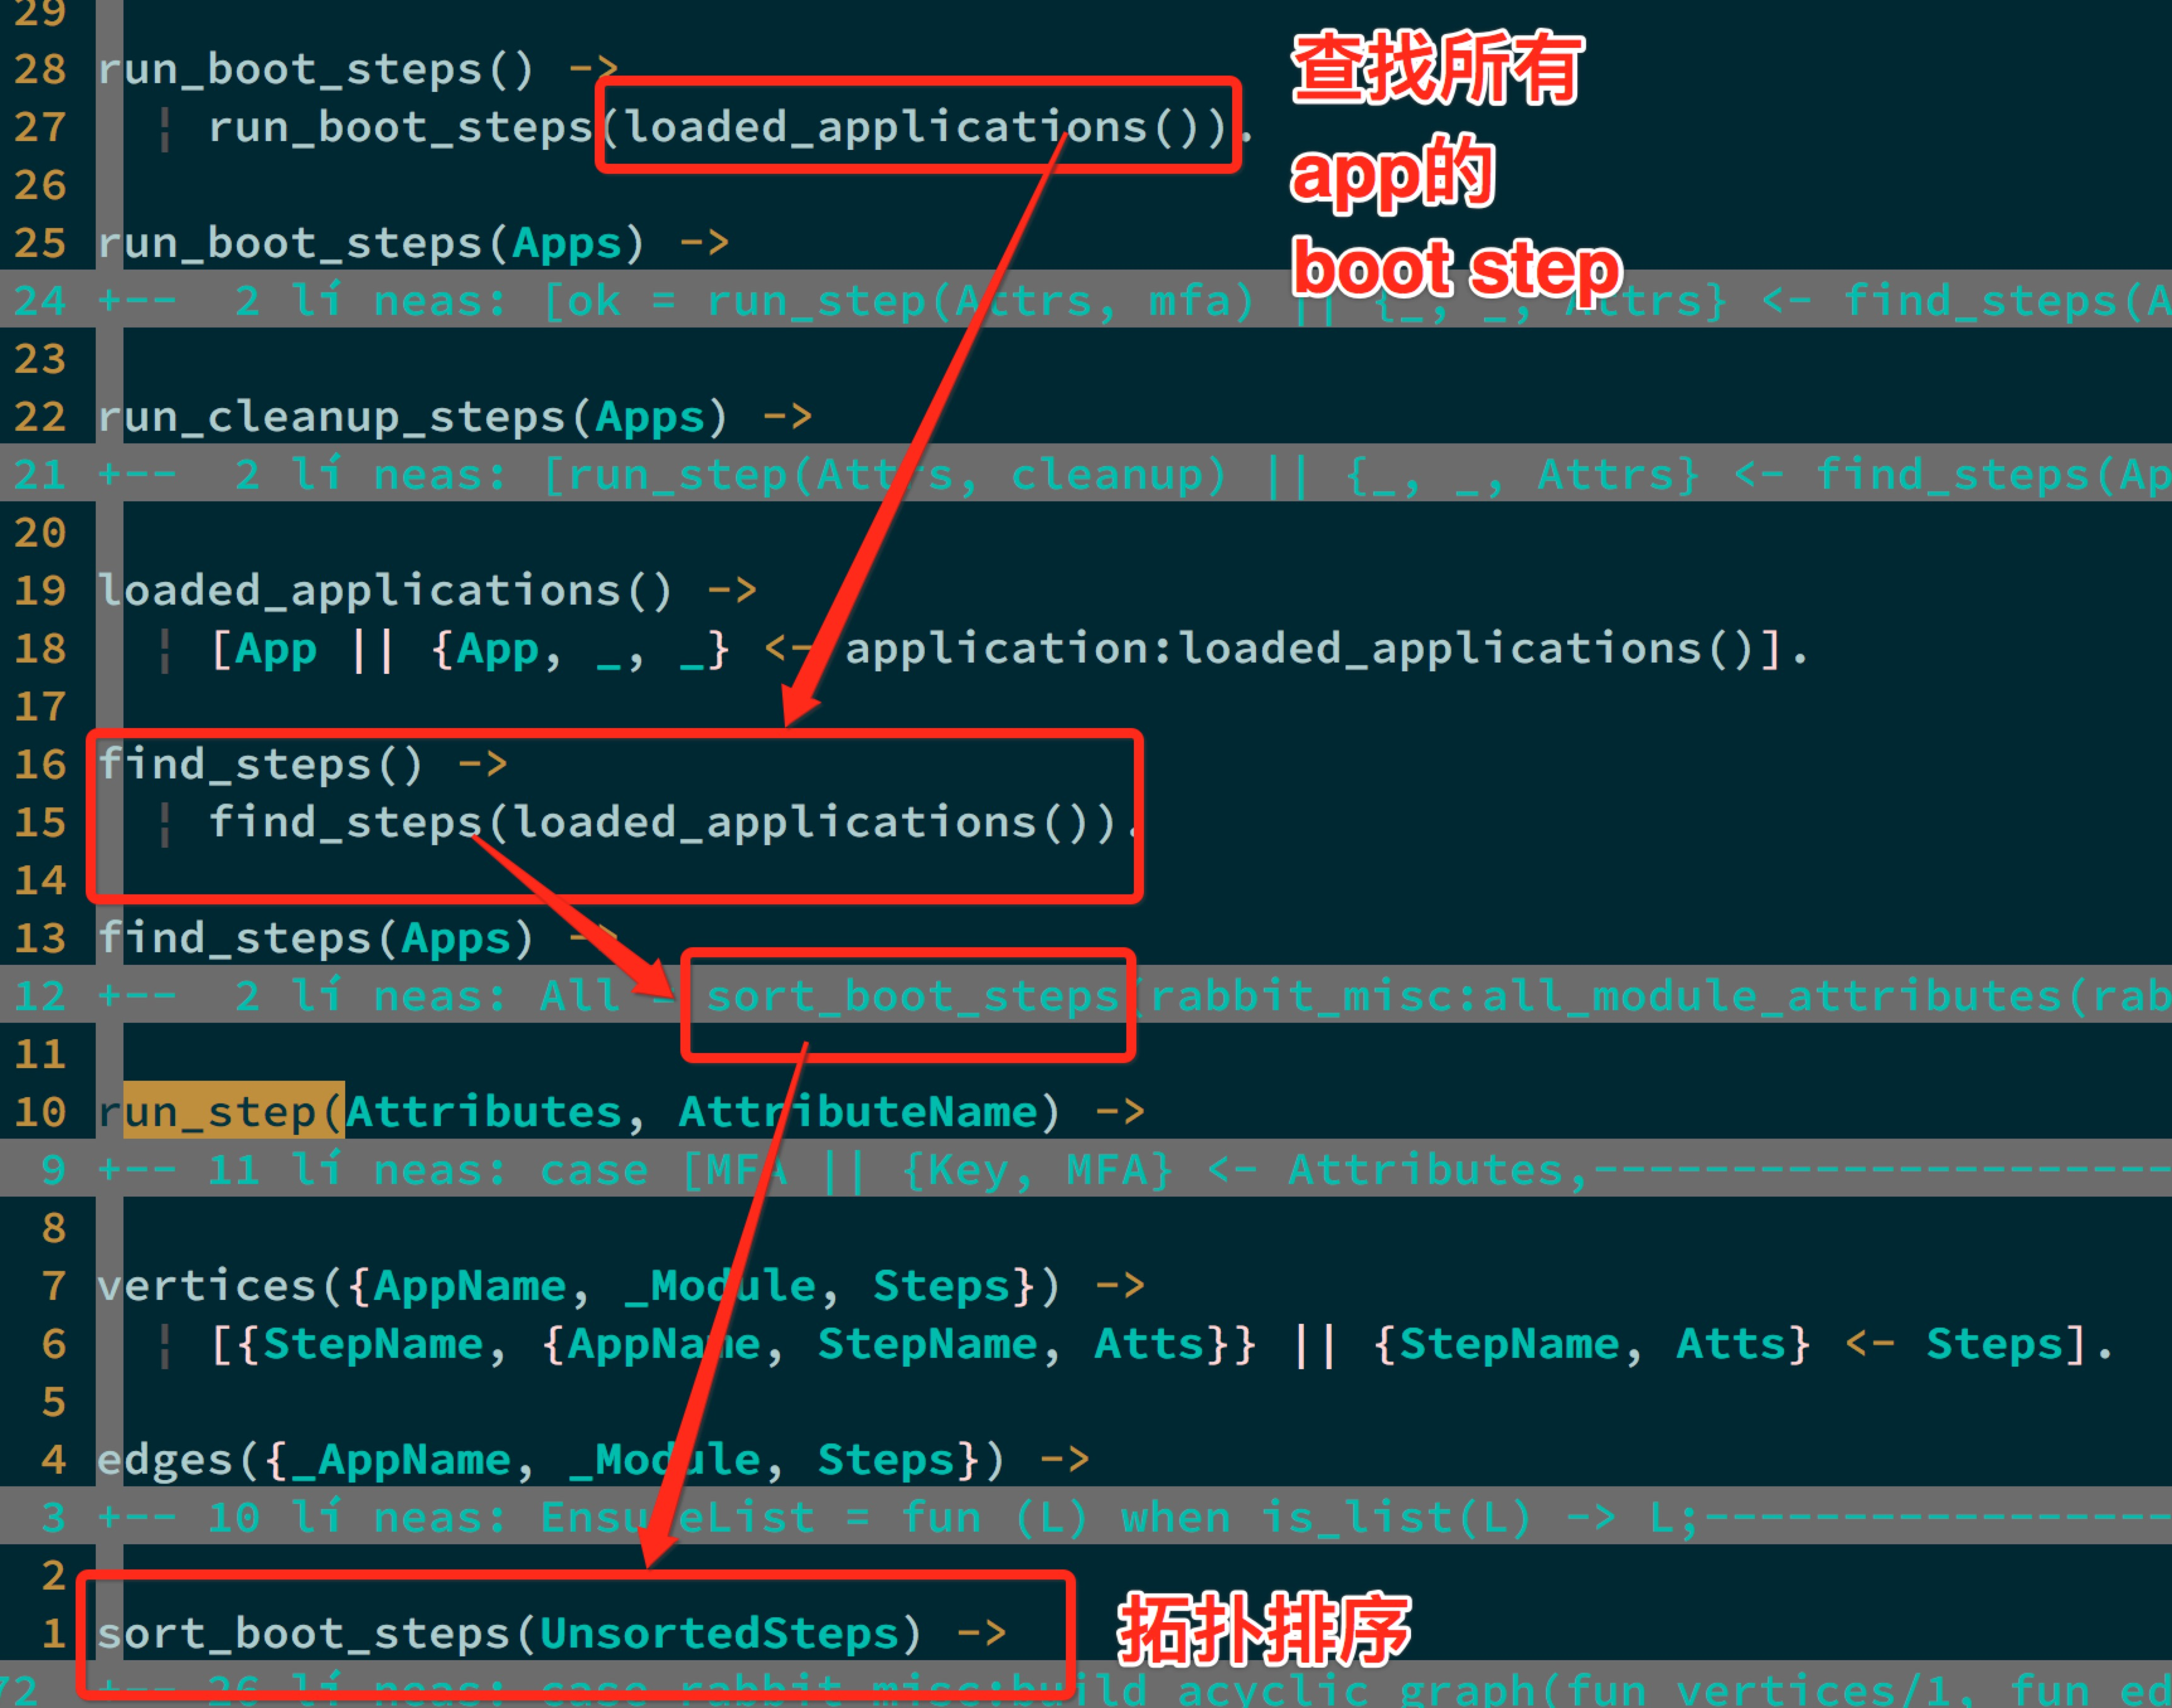
\includegraphics[width=\textwidth]{img/ch1/run_step.jpeg}
	\caption{\label{Fig:ch1/run_step}rabbit\_run\_steps.erl}
\end{figure}

这里为什么要用boot\_step的方式, 而不是一行一行的按顺序编写? 个人觉得主要是这种方式灵活, 解耦解得比较干净, 当需要给rabbitmq增加一个新的plugin时,也只需要编写自己的app即可。

顺便说下DAG,DAG可以在很多地方进行类似的优化;比如编译原理中代码块的DAG优化、spark中基于DAG的多stage优化了Hadoop的two stage;我们soa服务搞不清依赖关系时其实也可以通过DAG拓扑排序来理顺。





